\begin{document}
\graphicspath{ {images/frvt/} }

\section{Parameter Learning - Finite Random Variables and Trees}

\subsection{Generalizing Parameter Learning}

This section generalizes the ideas we've seen with parameter learning for a biased coin and for naive Bayes, specifically for maximum likelihood (so, no Laplace smoothing now). Specifically we look at learning parameters for a general finite random variable (for which estimating the bias of a coin is a special case) and learning all the potential tables in a tree-structured graphical model (for which naive Bayes is a special case).

For the finite random variable case, our derivation will revisit information measures from earlier in the course: entropy and information divergence. We'll see that maximum likelihood estimation relates to what we've seen earlier in the course on histograms -- frequencies in which we see outcomes occur.

Learning all the potential tables in a tree-structured graphical model can be phrased in terms of learning parameters for a collection of finite random variables.

Unlike the bulk of our previous coverage of parameter learning, we won't be taking derivatives in this section!


\subsection{Parameter Learning for a Finite Random Variable}

Let's build off of our coin tossing example, where we had an underlying distribution $p_X$ with parameter $\theta$, the probability of heads. We now explicitly make there be two parameters $\theta _{\text {heads}}$ and $\theta _{\text {tails}}$. In the more general case when there are many outcomes, it will be easier to write out a parameter for every value a random variable can take on rather than a parameter for all but one of them. Thus, using the same representation trick we saw earlier:

\begin{eqnarray*}
p_{X}(x;\theta)&=&\theta_{\text{heads}}^{\mathbf{1}\{x=\text{heads}\}}\theta_{\text{tails}}^{\mathbf{1}\{x=\text{tails}\}}=\begin{cases}
\theta_{\text{heads}} & \text{if }x=\text{heads},\\
\theta_{\text{tails}} & \text{if }x=\text{tails}.
\end{cases}
\end{eqnarray*}

In particular, in the general case when random variable $X$ has alphabet $\mathcal{X}$, then

{\centering$p_{X}(x;\theta )=\prod _{a\in \mathcal{X}}\theta _{a}^{\mathbf{1}\{ x=a\} }.$ \par}

(In the coin tossing case, $\mathcal{X}=\{ \text {heads},\text {tails}\}$.)

The training data $X^{(1)},\dots ,X^{(n)}$ are again assumed to be drawn i.i.d. from the distribution $p_{X}(\cdot ;\theta )$, so that the likelihood for observed data $X^{(1)}=x^{(1)},\dots ,X^{(n)}=x^{(n)}$ is

{\centering$\prod _{i=1}^{n}p_{X}(x^{(i)};\theta )=\prod _{i=1}^{n}\bigg\{ \prod _{a\in \mathcal{X}}\theta _{a}^{\mathbf{1}\{ x^{(i)}=a\} }\bigg\} .$ \par}
 
The log likelihood is thus

{\centering$\log \prod _{i=1}^{n}p_{X}(x^{(i)};\theta )=\log \prod _{i=1}^{n}\bigg\{ \prod _{a\in \mathcal{X}}\theta _{a}^{\mathbf{1}\{ x^{(i)}=a\} }\bigg\} =\sum _{i=1}^{n}\sum _{a\in \mathcal{X}}\mathbf{1}\{ x^{(i)}=a\} \log \theta _{a}.$ \par}
 
Now we exchange the ordering of the summations on the right-hand side to get

{\centering$\text {log likelihood}=\sum _{a\in \mathcal{X}}\bigg[\sum _{i=1}^{n}\mathbf{1}\{ x^{(i)}=a\} \bigg]\log \theta _{a}.$ \par}
 
Note that the maximum likelihood estimate $\widehat{\theta }$ of all the parameters $\theta$ (now $\theta$ has a parameter$\theta _{a}$ for each possible value $a\in \mathcal{X}$) is precisely the solution to the following constrained optimization problem:

\begin{eqnarray*}
 &  & \widehat{\theta}=\arg\max_{\theta = \{ \theta_a \text{ for }a\in\mathcal{X} \}}\bigg\{\sum_{a\in\mathcal{X}}\bigg[\sum_{i=1}^{n}\mathbf{1}\{x^{(i)}=a\}\bigg]\log\theta_{a}\bigg\}\\
 &  & \qquad\text{subject to }\sum_{a\in\mathcal{X}}\theta_{a}=1,\text{ and }\theta_{a}\ge0\text{ for all }a\in\mathcal{X}.
\end{eqnarray*}

(Technical detail: If we didn't have the inequality constraints, then it's possible to solve this using a single Lagrange multiplier to enforce the equality constraint that $\sum _{a\in \mathcal{X}}\theta _{a}=1$. If you do this, you will in fact get the correct answer, but it's not straightforward showing why it is definitely the unique global maximum.)

Let's see how information-theoretic measures can help us. Let $\widehat{p}_{X}$ refer to the empirical distribution (this is the histogram of frequencies) of $X$ that we get from our training data $x^{(1)},\dots ,x^{(n)}$, so that $\widehat{p}_{X}(x)$ is precisely the fraction of times we saw $x$ in the training data:

{\centering$\widehat{p}_{X}(x)=\frac{1}{n}\sum _{i=1}^{n}\mathbf{1}\{ x^{(i)}=x\} .$ \par}
 
Then the log likelihood is

\begin{eqnarray*}
 &  & \log\text{likelihood}\\
 &  & =\sum_{a\in\mathcal{X}}\underbrace{\bigg[\sum_{i=1}^{n}\mathbf{1}\{x^{(i)}=a\}\bigg]}_{n\cdot\widehat{p}_{X}(a)}\log\underbrace{\theta_{a}}_{p_{X}(a;\theta)}\\
 &  & =\sum_{a\in\mathcal{X}}n\cdot\widehat{p}_{X}(a)\log p_{X}(a;\theta)\\
 &  & =\sum_{a\in\mathcal{X}}n\cdot\widehat{p}_{X}(a)\log\Big(p_{X}(a;\theta)\frac{\widehat{p}_{X}(a)}{\widehat{p}_{X}(a)}\Big)\\
 &  & =\sum_{a\in\mathcal{X}}n\cdot\widehat{p}_{X}(a)\Big(\log\widehat{p}_{X}(a)+\log\frac{p_{X}(a;\theta)}{\widehat{p}_{X}(a)}\Big)\\
 &  & =n\bigg[\sum_{a\in\mathcal{X}}\widehat{p}_{X}(a)\log\widehat{p}_{X}(a)+\sum_{a\in\mathcal{X}}\widehat{p}_{X}(a)\log\frac{p_{X}(a;\theta)}{\widehat{p}_{X}(a)}\bigg]\\
 &  & =n\big[-H(\widehat{p}_{X})-D\big(\widehat{p}_{X}\parallel p_{X}(\cdot;\theta)\big)\big]\\
 &  & =-n\big[H(\widehat{p}_{X})+D\big(\widehat{p}_{X}\parallel p_{X}(\cdot;\theta)\big)\big].
\end{eqnarray*}

Note that here we are using natural log with entropy and information divergence instead of log base 2 -- this is actually commonly done and just results in the overall quantity being scaled by a constant (since $\log _2 x = \frac{\log x}{\log 2}$). Recall that when we used log base 2, we measured information content in terms of bits. When using natural log, information content is measured in terms of what are called nats.

Importantly, note that to maximize the likelihood, the only expression that depends on $\theta$ here is the divergence, and in particular, maximizing the likelihood is the same as (because of the minus sign in the last expression) minimizing the divergence $D\big (\widehat{p}_{X}\parallel p_{X}(\cdot ;\theta )\big )$. Here, since we treat our training data as fixed, then $\widehat{p}_{X}$ is a fixed distribution, and so minimizing the divergence means choosing a distribution $p_{X}(\cdot ;\theta )$. But we know from Gibbs' inequality what the best choice of $p_{X}(\cdot ;\theta )$ is! In particular, the divergence is the smallest possible and, in particular, 0 when $p_{X}(\cdot ;\theta )$ is set to be equal to the empirical distribution $\widehat{p}_{X}$, so we set

{\centering$\underbrace{p_{X}(a;\theta )}_{\theta _{a}}=\widehat{p}_{X}(a)\qquad \text {for all }a\in \mathcal{X}.$ \par}
 
So the maximum likelihood estimate $\widehat{\theta }_{a}$ for parameter $\theta _{a}$ is the fraction of times we see $a$ in the training data $x^{(1)},\dots ,x^{(n)}$. Note that Gibbs' inequality tells us that we cannot do better. The unique global maximum is to choose $\widehat{\theta }_{a}=\widehat{p}_{X}(a)$ for all $a\in \mathcal{X}$. There is no need to check second derivatives, boundaries, etc. (Technical note: When we have more than a single variable, justifying whether a point is a local maximum in general requires more work than in the single variable calculus case since there could be saddle points. However, in this case, Gibbs' inequality tells us that there's a unique maximum.)


\subsection{Parameter Learning for an Undirected Tree-Structured Graphical Model}

We now look at how to learn potential tables for a tree-structured graphical model. Recall that for the exact same distribution, the way in which we specify potential tables is not unique (i.e., there could be multiple way to specify potential tables to represent the same distribution). This is fine. We can still learn potential tables systematically with maximum likelihood. In fact, we did this already when we trained a naive Bayes classifier! Let's build some intuition from the naive Bayes classifier case (again, we stick to maximum likelihood here -- no Laplace smoothing). The graphical model was as follows:

{\centering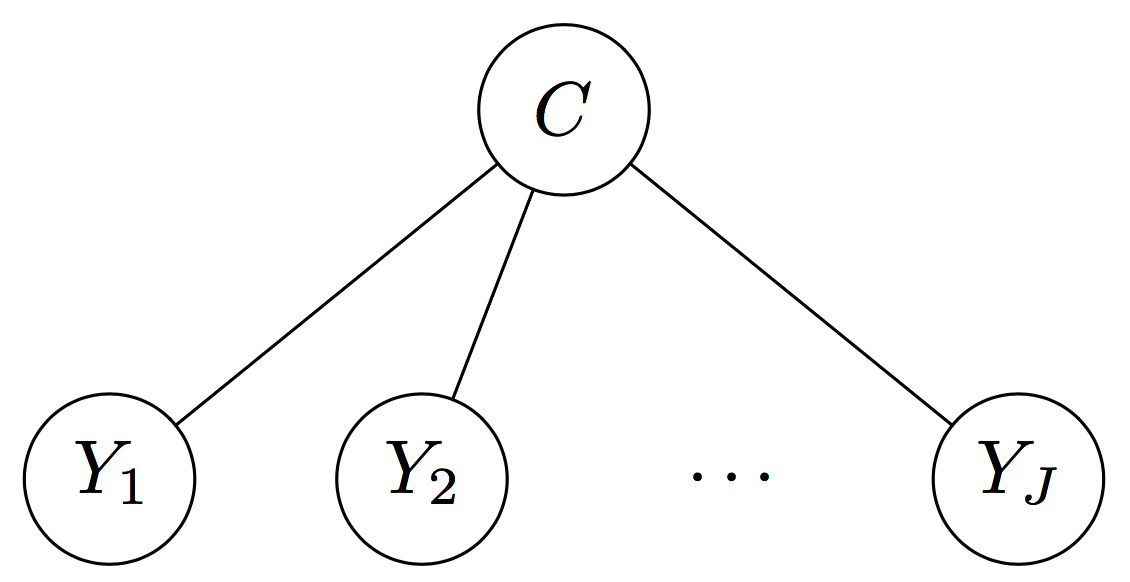
\includegraphics[scale=0.3]{images_naive-bayes} \par}

How we learned the parameters was that we treated node $C$ as the root node. Then the factorization was

{\centering$\underbrace{p_{C}(c;\theta )}_{\text {1 potential table}}\underbrace{\prod _{j=1}^{J}p_{Y_{j}\mid C}(y_{j}\mid c;\theta )}_{J\text { potential tables}}.$ \par}
 
Each of the potential tables is actually specified in terms of different parameters. In particular, $p_C$ only depends on parameter $s$, and $p_{Y_{j}\mid C}$ only depends on $p_j$ and $q_j$.

What we did was we estimated $p_{C}(\cdot ;\theta )$ with the empirical distribution

{\centering$\widehat{p}_{C}(c)=\text {fraction of times in training data we see label }c=\frac{1}{n}\sum _{i=1}^{n}\mathbf{1}\{ c^{(i)}=c\} .$ \par}
 
When $c=\text {spam}$, we called this parameter $s$. Of course when $c=\text {ham}$, then this parameter is just $1-s$, which we didn't have to separately store.

We estimated $p_{Y_{j}\mid C}(\cdot \mid c;\theta )$ with the empirical conditional distribution

{\centering{\renewcommand{\arraystretch}{1.5}
\begin{tabular}{r c l}
$\widehat{p}_{Y_{j}\mid C}(y_{j}\mid c)$ & $=$ & $\text {fraction of times in training data we see }y_{j}\text { amongst emails with label }c$ \\
  & $=$ & $\frac{\sum _{i=1}^{n}\mathbf{1}\{ y_{j}^{(i)}=y_{j},c^{(i)}=c\} }{\sum _{i=1}^{n}\mathbf{1}\{ c^{(i)}=c\} }.$ 
\end{tabular}} \par}

When $c=\text {ham}$, we called this parameter $p_j$. When $c=\text {spam}$, we called this parameter $q_j$.

For the general case of learning maximum likelihood parameters for a given tree-structured graphical model, we can choose an arbitrary root node (which has a node potential table corresponding to the probability of the root node) and then treat the edge potential tables as conditional probability distributions. For the root node, we estimate its node potential table with the empirical distribution for just that node. For the other potential tables, we estimate them using empirical conditional distributions. Let me walk through a specific example. Consider the following graphical model:

{\centering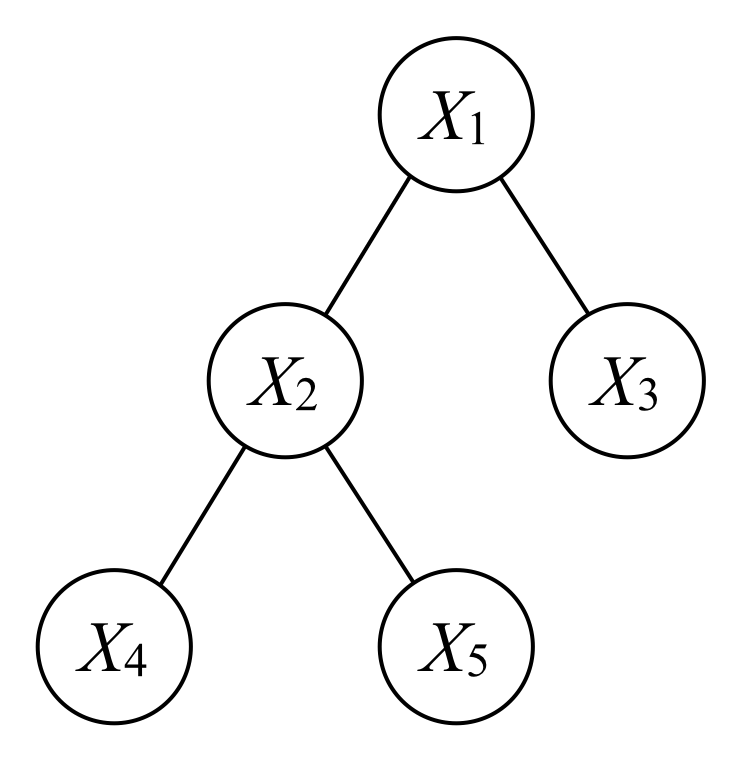
\includegraphics[scale=0.3]{images_sec-graphical-models-five-node-example} \par}

We assume we have access to training data

{\centering$\underbrace{X_{1}^{(1)},X_{2}^{(1)},X_{3}^{(1)},X_{4}^{(1)},X_{5}^{(1)}}_{\text {first training data point}},\quad \underbrace{X_{1}^{(2)},X_{2}^{(2)},X_{3}^{(2)},X_{4}^{(2)},X_{5}^{(2)}}_{\text {second training data point}},\quad \dots ,\quad \underbrace{X_{1}^{(n)},X_{2}^{(n)},X_{3}^{(n)},X_{4}^{(n)},X_{5}^{(n)}}_{n\text {-th training data point}}.$ \par}
 
The likelihood is

{\centering$\prod _{i=1}^{n}p_{X_{1},X_{2},X_{3},X_{4},X_{5}}(x_{1}^{(i)},x_{2}^{(i)},x_{3}^{(i)},x_{4}^{(i)},x_{5}^{(i)};\theta ).$ \par}
 
By choosing node 1 arbitrarily as the root, then we write $p_{X_{1},X_{2},X_{3},X_{4},X_{5}}(\cdot ;\theta )$ as

{\centering$\underbrace{p_{X_{1},X_{2},X_{3},X_{4},X_{5}}}_{\text {parameters }\theta }=\underbrace{p_{X_{1}}}_{\text {parameters }\theta _{1}}\underbrace{p_{X_{2}\mid X_{1}}}_{\theta _{2\mid 1}}\underbrace{p_{X_{3}\mid X_{1}}}_{\theta _{3\mid 1}}\underbrace{p_{X_{4}\mid X_{2}}}_{\theta _{4\mid 2}}\underbrace{p_{X_{5}\mid X_{2}}}_{\theta _{5\mid 2}},$ \par}
 
where we use $\theta _{1},\theta _{2\mid 1},\theta _{3\mid 1},\theta _{4\mid 2},\theta _{5\mid 2}$ to refer to parameters for each of the tables that we aim to learn. The notation here is going to be a bit messy. We'll use the notation

{\centering$\theta _{1;a}\triangleq p_{X_{1}}(a;\theta )$ \par}
 
{\centering$\theta _{2\mid 1;a\mid b}\triangleq p_{X_{2}\mid X_{1}}(a\mid b;\theta _{2\mid 1})$ \par}
 
and so forth.

We assume these parameters to be separate from each other (so that similar to the naive Bayes case, we can learn each of these tables separately). Then the log likelihood is

\begin{eqnarray*}
 &  & \log\prod_{i=1}^{n}p_{X_{1},X_{2},X_{3},X_{4},X_{5}}(x_{1}^{(i)},x_{2}^{(i)},x_{3}^{(i)},x_{4}^{(i)},x_{5}^{(i)};\theta)\\
 &  & =\log\prod_{i=1}^{n}\big\{ p_{X_{1}}(x_{1}^{(i)};\theta_{1})p_{X_{2}\mid X_{1}}(x_{2}^{(i)}\mid x_{1}^{(i)};\theta_{2\mid1})p_{X_{3}\mid X_{1}}(x_{3}^{(i)}\mid x_{1}^{(i)};\theta_{3\mid1}) \\
 &  & \qquad\qquad\;\; p_{X_{4}\mid X_{2}}(x_{4}^{(i)}\mid x_{2}^{(i)};\theta_{4\mid2})p_{X_{5}\mid X_{2}}(x_{5}^{(i)}\mid x_{2}^{(i)};\theta_{5\mid2})\big\}\\
 &  & =\text{log likelihood for }X_{1}\text{ with parameter }\theta_{1}\\
 &  & \quad+\sum_{a}\mathbf{1}\{x_{1}^{(i)}=a\}\cdot(\text{log likelihood for }X_{2}\mid X_{1}=a\text{ with parameter }\theta_{2\mid1})\\
 &  & \quad+\sum_{a}\mathbf{1}\{x_{1}^{(i)}=a\}\cdot(\text{log likelihood for }X_{3}\mid X_{1}=a\text{ with parameter }\theta_{3\mid1})\\
 &  & \quad+\sum_{a}\mathbf{1}\{x_{2}^{(i)}=a\}\cdot(\text{log likelihood for }X_{4}\mid X_{2}=a\text{ with parameter }\theta_{4\mid2})\\
 &  & \quad+\sum_{a}\mathbf{1}\{x_{2}^{(i)}=a\}\cdot(\text{log likelihood for }X_{5}\mid X_{2}=a\text{ with parameter }\theta_{5\mid2})
\end{eqnarray*}

To maximize the overall log likelihood, we maximize the log likelihood for each of the five tables separately, where the root node corresponds to learning the parameter for a single finite random variable, whereas for each of the edges, we learn a finite random variable for every possible value that we are conditioning on. In both of these cases, the result from parameter learning for a finite random variable (for maximum likelihood) says that the ML estimate corresponds to fitting an empirical distribution.

Thus, for the root node, we have

{\centering$\widehat{\theta }_{1;a}=\widehat{p}_{X_{1}}(a)=\frac{1}{n}\sum _{i=1}^{n}\mathbf{1}\{ x_{1}^{(i)}=a\} ,$ \par}
 
and for the conditional probability tables, we have

{\centering$\widehat{\theta}_{i\mid j;a\mid b} = \widehat{p}_{X_{i}\mid X_{j}}(a\mid b)=\frac{\sum_{\ell=1}^{n}\mathbf{1}\{x_{i}^{(\ell)}=a,x_{j}^{(\ell)}=b\}}{\sum_{\ell=1}^{n}\mathbf{1}\{x_{j}^{(\ell)}=b\}}.$ \par}

Note that if we chose the root node to be some other node, of course, the factorization we get would be different, which means that the tables we are learning will be different but will represent the same distribution.


\end{document}
